% Drawing 154/08-2 -- folder 154, batch 08, archive page 142 (PDF page 143).
% Transcription: page de dessins à l'encre. En haut à gauche, un rectangle partagé par deux droites horizontales, les colonnes marquées en haut $A\,B\,C\,D\,E\,F\,G\,H$ (flèche vers la droite) et en bas $H\,G\,F\,E\,D\,C\,B\,A$ (lecture de l'avant-dernière lettre incertaine), une flèche vers le bas à gauche. Au milieu, un arbre binaire de flèches issu de $D\,E\,F\,G$ ; un fuseau allongé traversé de droites ; un croisement de deux droites sur deux horizontales. En haut à droite, un diagramme en « fils » : sept fils verticaux $A, B, C, D, E, F, G$ qui se croisent deux à deux, sur un réseau de lignes horizontales numérotées à droite $1$ à $11$ et à gauche $1'$ à $9'$ ; en bas, l'ordre d'arrivée $G\,A\,E\,D\,C\,F\,B$. En bas à droite, le même principe sur un quadrillage, colonnes $A$ à $G$, lignes $1$ à $11$, l'arrivée marquée $G\,A$. En bas au milieu, un cylindre dont le bord supérieur porte $G, F, E, D$ et $A, B, C$, le bord inférieur $D, E, F$ et $B, A, G$
% Kind: wiring diagrams (columns A ... H, rows numbered); rectangle with letters; spindle; cylinder. Method 2 (schematic redraw from the facsimile). Status: partial.
% Notes: Page of ink drawings over a printed job banner (not reproduced), read from the page view. Top left, a rectangle divided by two horizontal lines, columns marked A B C D E F G H at the top (arrow to the right) and H G F E D C B A at the bottom. Top right and middle right: two wiring diagrams, strands A ... G running down through rows numbered 1 to 11, crossing in pairs (some crossings thickened, arrows on a few strands), the order at the foot read « G A E D C F B » and « G A ». A small tree of arrows from D E F G, a spindle with marked vertices, crossings on two lines with a dark mark, and an elliptical cylinder with letters A ... G round it. The wiring diagrams are drawn as grids with their main crossings only; the crossing sequence is not encoded, as several crossings are overinked and cannot be read with certainty at this resolution.
% Coordinates: 1 unit = 1 mm = 1/100 of the crop width (bbox in page fractions: [0.125, 0.092, 0.927, 0.502]).
% Redrawn by Claude (claude-opus-5-5), issue #73, 2026-11-07; not checked by a human; not compiled (no TeX in the session).
% Rights: reproduces part of the work -- behind RENDER_TRANSCRIPTS, never published by itself.
\documentclass[tikz,border=3pt]{standalone}
\usepackage{amsmath,amssymb}
\usetikzlibrary{patterns,arrows.meta}
\tikzset{Or/.style={orange!90!black}, Ye/.style={yellow!80!orange}, Lg/.style={green!60!black!70}, Dg/.style={green!45!black}, Br/.style={brown!80!black}, Rd/.style={red!85!black}, Bl/.style={blue!70!black}, Gy/.style={black!40}, pencil/.style={black!45}, struck/.style={black!35}, mark/.style={circle,draw,inner sep=1.3pt}, pt/.style={circle,fill,inner sep=0.9pt}, opt/.style={circle,draw,fill=white,inner sep=1.1pt}}
\begin{document}
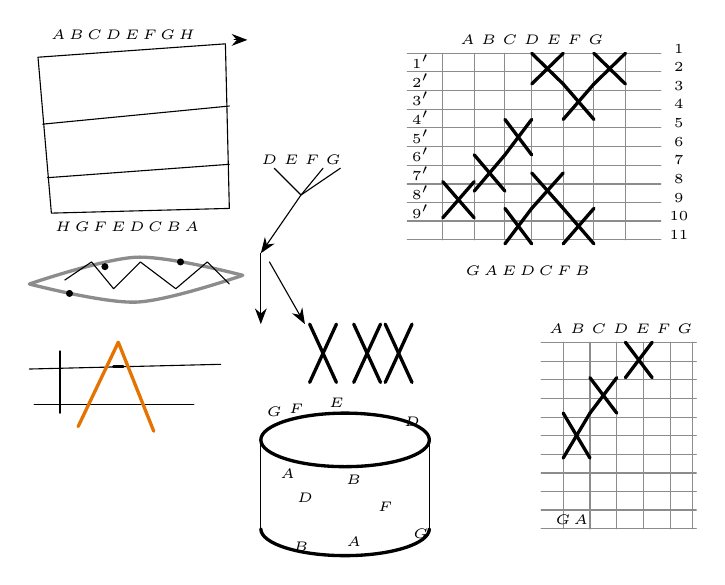
\begin{tikzpicture}[x=1mm,y=1mm,line cap=round,line join=round,font=\scriptsize]
\draw (2.8,-4.5) -- (26.6,-2.8) -- (27.1,-23.7) -- (4.5,-24.3) -- cycle;
\draw (3.4,-13) -- (27.1,-10.7);
\draw (4,-19.8) -- (27.1,-18.1);
\node[inner sep=1pt] at (13.6,-1.7) {\tiny $A\,B\,C\,D\,E\,F\,G\,H$};
\draw[-{Stealth[length=2mm]}] (27.7,-2.3) -- (29.4,-2.3);
\node[inner sep=1pt] at (14.1,-26) {\tiny $H\,G\,F\,E\,D\,C\,B\,A$};
\draw[pencil] (49.7,-4) -- (81.9,-4);
\draw[pencil] (49.7,-6.3) -- (81.9,-6.3);
\draw[pencil] (49.7,-8.7) -- (81.9,-8.7);
\draw[pencil] (49.7,-11.1) -- (81.9,-11.1);
\draw[pencil] (49.7,-13.4) -- (81.9,-13.4);
\draw[pencil] (49.7,-15.8) -- (81.9,-15.8);
\draw[pencil] (49.7,-18.2) -- (81.9,-18.2);
\draw[pencil] (49.7,-20.6) -- (81.9,-20.6);
\draw[pencil] (49.7,-22.9) -- (81.9,-22.9);
\draw[pencil] (49.7,-25.3) -- (81.9,-25.3);
\draw[pencil] (49.7,-27.7) -- (81.9,-27.7);
\draw[pencil] (54.2,-4) -- (54.2,-27.7);
\draw[pencil] (58.2,-4) -- (58.2,-27.7);
\draw[pencil] (62.1,-4) -- (62.1,-27.7);
\draw[pencil] (65.5,-4) -- (65.5,-27.7);
\draw[pencil] (69.5,-4) -- (69.5,-27.7);
\draw[pencil] (73.4,-4) -- (73.4,-27.7);
\draw[pencil] (77.4,-4) -- (77.4,-27.7);
\node[inner sep=1pt] at (65.5,-2.3) {\tiny $A\ B\ C\ D\ E\ F\ G$};
\draw[very thick] (65.5,-4) -- (69.5,-7.9);
\draw[very thick] (69.5,-4) -- (65.5,-7.9);
\draw[very thick] (73.4,-4) -- (77.4,-7.9);
\draw[very thick] (77.4,-4) -- (73.4,-7.9);
\draw[very thick] (69.5,-7.9) -- (73.4,-12.4);
\draw[very thick] (73.4,-7.9) -- (69.5,-12.4);
\draw[very thick] (62.1,-12.4) -- (65.5,-16.9);
\draw[very thick] (65.5,-12.4) -- (62.1,-16.9);
\draw[very thick] (58.2,-16.9) -- (62.1,-21.5);
\draw[very thick] (62.1,-16.9) -- (58.2,-21.5);
\draw[very thick] (65.5,-19.2) -- (69.5,-23.7);
\draw[very thick] (69.5,-19.2) -- (65.5,-23.7);
\draw[very thick] (62.1,-23.7) -- (65.5,-28.2);
\draw[very thick] (65.5,-23.7) -- (62.1,-28.2);
\draw[very thick] (69.5,-23.7) -- (73.4,-28.2);
\draw[very thick] (73.4,-23.7) -- (69.5,-28.2);
\draw[very thick] (54.2,-20.3) -- (58.2,-24.9);
\draw[very thick] (58.2,-20.3) -- (54.2,-24.9);
\node[inner sep=1pt] at (51.4,-5.1) {\tiny $1'$};
\node[inner sep=1pt] at (51.4,-7.5) {\tiny $2'$};
\node[inner sep=1pt] at (51.4,-9.8) {\tiny $3'$};
\node[inner sep=1pt] at (51.4,-12.2) {\tiny $4'$};
\node[inner sep=1pt] at (51.4,-14.6) {\tiny $5'$};
\node[inner sep=1pt] at (51.4,-16.9) {\tiny $6'$};
\node[inner sep=1pt] at (51.4,-19.3) {\tiny $7'$};
\node[inner sep=1pt] at (51.4,-21.7) {\tiny $8'$};
\node[inner sep=1pt] at (51.4,-24.1) {\tiny $9'$};
\node[inner sep=1pt] at (84.2,-3.4) {\tiny $1$};
\node[inner sep=1pt] at (84.2,-5.8) {\tiny $2$};
\node[inner sep=1pt] at (84.2,-8.1) {\tiny $3$};
\node[inner sep=1pt] at (84.2,-10.5) {\tiny $4$};
\node[inner sep=1pt] at (84.2,-12.9) {\tiny $5$};
\node[inner sep=1pt] at (84.2,-15.3) {\tiny $6$};
\node[inner sep=1pt] at (84.2,-17.6) {\tiny $7$};
\node[inner sep=1pt] at (84.2,-20) {\tiny $8$};
\node[inner sep=1pt] at (84.2,-22.4) {\tiny $9$};
\node[inner sep=1pt] at (84.2,-24.7) {\tiny $10$};
\node[inner sep=1pt] at (84.2,-27.1) {\tiny $11$};
\node[inner sep=1pt] at (65,-31.6) {\tiny $G\,A\,E\,D\,C\,F\,B$};
\draw[pencil] (66.7,-40.7) -- (86.4,-40.7);
\draw[pencil] (66.7,-43.1) -- (86.4,-43.1);
\draw[pencil] (66.7,-45.4) -- (86.4,-45.4);
\draw[pencil] (66.7,-47.8) -- (86.4,-47.8);
\draw[pencil] (66.7,-50.2) -- (86.4,-50.2);
\draw[pencil] (66.7,-52.5) -- (86.4,-52.5);
\draw[pencil] (66.7,-54.9) -- (86.4,-54.9);
\draw[pencil] (66.7,-57.3) -- (86.4,-57.3);
\draw[pencil] (66.7,-59.7) -- (86.4,-59.7);
\draw[pencil] (66.7,-62) -- (86.4,-62);
\draw[pencil] (66.7,-64.4) -- (86.4,-64.4);
\draw[pencil] (69.5,-40.7) -- (69.5,-64.4);
\draw[pencil] (72.9,-40.7) -- (72.9,-64.4);
\draw[pencil] (76.3,-40.7) -- (76.3,-64.4);
\draw[pencil] (79.7,-40.7) -- (79.7,-64.4);
\draw[pencil] (83.1,-40.7) -- (83.1,-64.4);
\draw[pencil] (85.9,-40.7) -- (85.9,-64.4);
\node[inner sep=1pt] at (76.8,-39) {\tiny $A\ B\ C\ D\ E\ F\ G$};
\draw[very thick] (77.4,-40.7) -- (80.8,-45.2);
\draw[very thick] (80.8,-40.7) -- (77.4,-45.2);
\draw[very thick] (69.5,-49.7) -- (72.9,-55.4);
\draw[very thick] (72.9,-49.7) -- (69.5,-55.4);
\draw[very thick] (72.9,-45.2) -- (76.3,-49.7);
\draw[very thick] (76.3,-45.2) -- (72.9,-49.7);
\node[inner sep=1pt] at (70.6,-63.3) {\tiny $G\,A$};
\draw[-{Stealth[length=2mm]}] (32.8,-18.6) -- (36.2,-22) -- (31.1,-29.4);
\draw (39,-18.6) -- (36.2,-22);
\draw (41.2,-18.6) -- (36.2,-22);
\node[inner sep=1pt] at (36.2,-17.5) {\tiny $D\ E\ F\ G$};
\draw[-{Stealth[length=2mm]}] (31.1,-29.4) -- (31.1,-38.4);
\draw[-{Stealth[length=2mm]}] (32.2,-30.5) -- (36.7,-38.4);
\draw[pencil,very thick] plot[smooth, tension=0.55] coordinates {(1.7,-33.3) (15.3,-29.9) (28.8,-32.2)};
\draw[pencil,very thick] plot[smooth, tension=0.55] coordinates {(1.7,-33.3) (15.3,-35.6) (28.8,-32.2)};
\draw (6.2,-32.8) -- (9.6,-30.5) -- (12.4,-33.9) -- (15.8,-30.5) -- (20.3,-33.9) -- (24.3,-30.5) -- (27.1,-33.3);
\node[pt] at (6.8,-34.5) {};
\node[pt] at (11.3,-31.1) {};
\node[pt] at (20.9,-30.5) {};
\draw (1.7,-44.1) -- (26,-43.5);
\draw (2.3,-48.6) -- (22.6,-48.6);
\draw[Or,very thick] (7.9,-51.4) -- (13,-40.7);
\draw[Or,very thick] (13,-40.7) -- (17.5,-52);
\draw (5.6,-41.8) -- (5.6,-49.7);
\draw[very thick] (12.4,-43.8) -- (13.6,-43.8);
\draw[very thick] (37.3,-38.4) -- (40.7,-45.8);
\draw[very thick] (40.7,-38.4) -- (37.3,-45.8);
\draw[very thick] (42.9,-38.4) -- (46.3,-45.8);
\draw[very thick] (46.3,-38.4) -- (42.9,-45.8);
\draw[very thick] (46.9,-38.4) -- (50.3,-45.8);
\draw[very thick] (50.3,-38.4) -- (46.9,-45.8);
\draw[very thick] (41.8,-53.1) ellipse[x radius=10.7, y radius=3.4];
\draw[very thick] (31.1,-64.4) arc[start angle=180, end angle=360, x radius=10.7, y radius=3.4];
\draw (31.1,-53.1) -- (31.1,-64.4);
\draw (52.5,-53.1) -- (52.5,-64.4);
\node[inner sep=1pt] at (32.8,-49.5) {\tiny $G$};
\node[inner sep=1pt] at (35.6,-49.2) {\tiny $F$};
\node[inner sep=1pt] at (40.7,-48.4) {\tiny $E$};
\node[inner sep=1pt] at (50.3,-50.8) {\tiny $D$};
\node[inner sep=1pt] at (34.5,-57.4) {\tiny $A$};
\node[inner sep=1pt] at (42.9,-58.2) {\tiny $B$};
\node[inner sep=1pt] at (36.7,-60.5) {\tiny $D$};
\node[inner sep=1pt] at (46.9,-61.6) {\tiny $F$};
\node[inner sep=1pt] at (36.2,-66.7) {\tiny $B$};
\node[inner sep=1pt] at (42.9,-66.1) {\tiny $A$};
\node[inner sep=1pt] at (51.4,-65) {\tiny $G$};
\end{tikzpicture}
\end{document}
